

\def \currentAuthor {Lukas Vogel} %so kann jederzeit der Autor geändert werden -> wird in der Fusszeile angezeigt.



\chapter*{Notationen}
Beschreibung wie Code, Hinweise, Zitate etc. formatiert werden  

\chapter{Einleitung}
Diese Diplomarbeit befasst sich mit der Entwicklung des Prototyps: NeXt. Das Produkt ist eine spielbare Version eines Computerspiels in dem sogenannte Jump and Run-Elemente, Puzzele-Elemente sowie Zeitmanagement-Elemente beinhaltet sind. Das Projekt wurde in Verbindung mit der Firma ClockStone Softwareentwicklung GmbH. erarbeitet. Interesse könnte diese Dokumentation bei jedem erwecken,	 der sich über Spielentwicklung in Verbindung mit der Unity-Engine  informieren will. Des Weiteren werden auch die Aspekte des Projektmanagements dieser Arbeit dargelegt.  

\chapter{Projektmanagement}

\section{Metainformationen}
\subsection{Team}
\begin{table}[H]
		\caption{Team}
	\renewcommand{\arraystretch}{1.5}
	\begin{tabular}{|p{8cm}|p{8cm}|}
		\hline
		\includegraphics[width=6cm]{images/vogelBeisp.jpg}
		\caption{Leitner}
		\label{leitner}
		 & 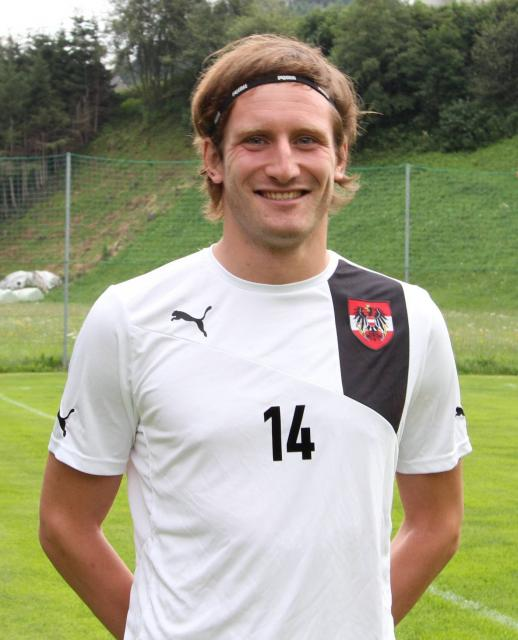
\includegraphics[width=6cm]{images/leitnerBeisp.jpg}
		 \caption{Vogel}
		 \label{Vogel}
		 \\
		\hline
		Team-Leiter & Teammitglied\\
		\hline
		Lukas Vogel & Leitner Michael\\
		\hline
	\end{tabular}
\end{table}
\subsection{Betreuer}
Seitens der Schule hat sich Herr Claudio Landerer bereiterklärt unser Projekt zu Betreuen. Er brachte uns in seinem Unterricht das Programmieren bei. 
	\begin{figure}[H]
		\centering
		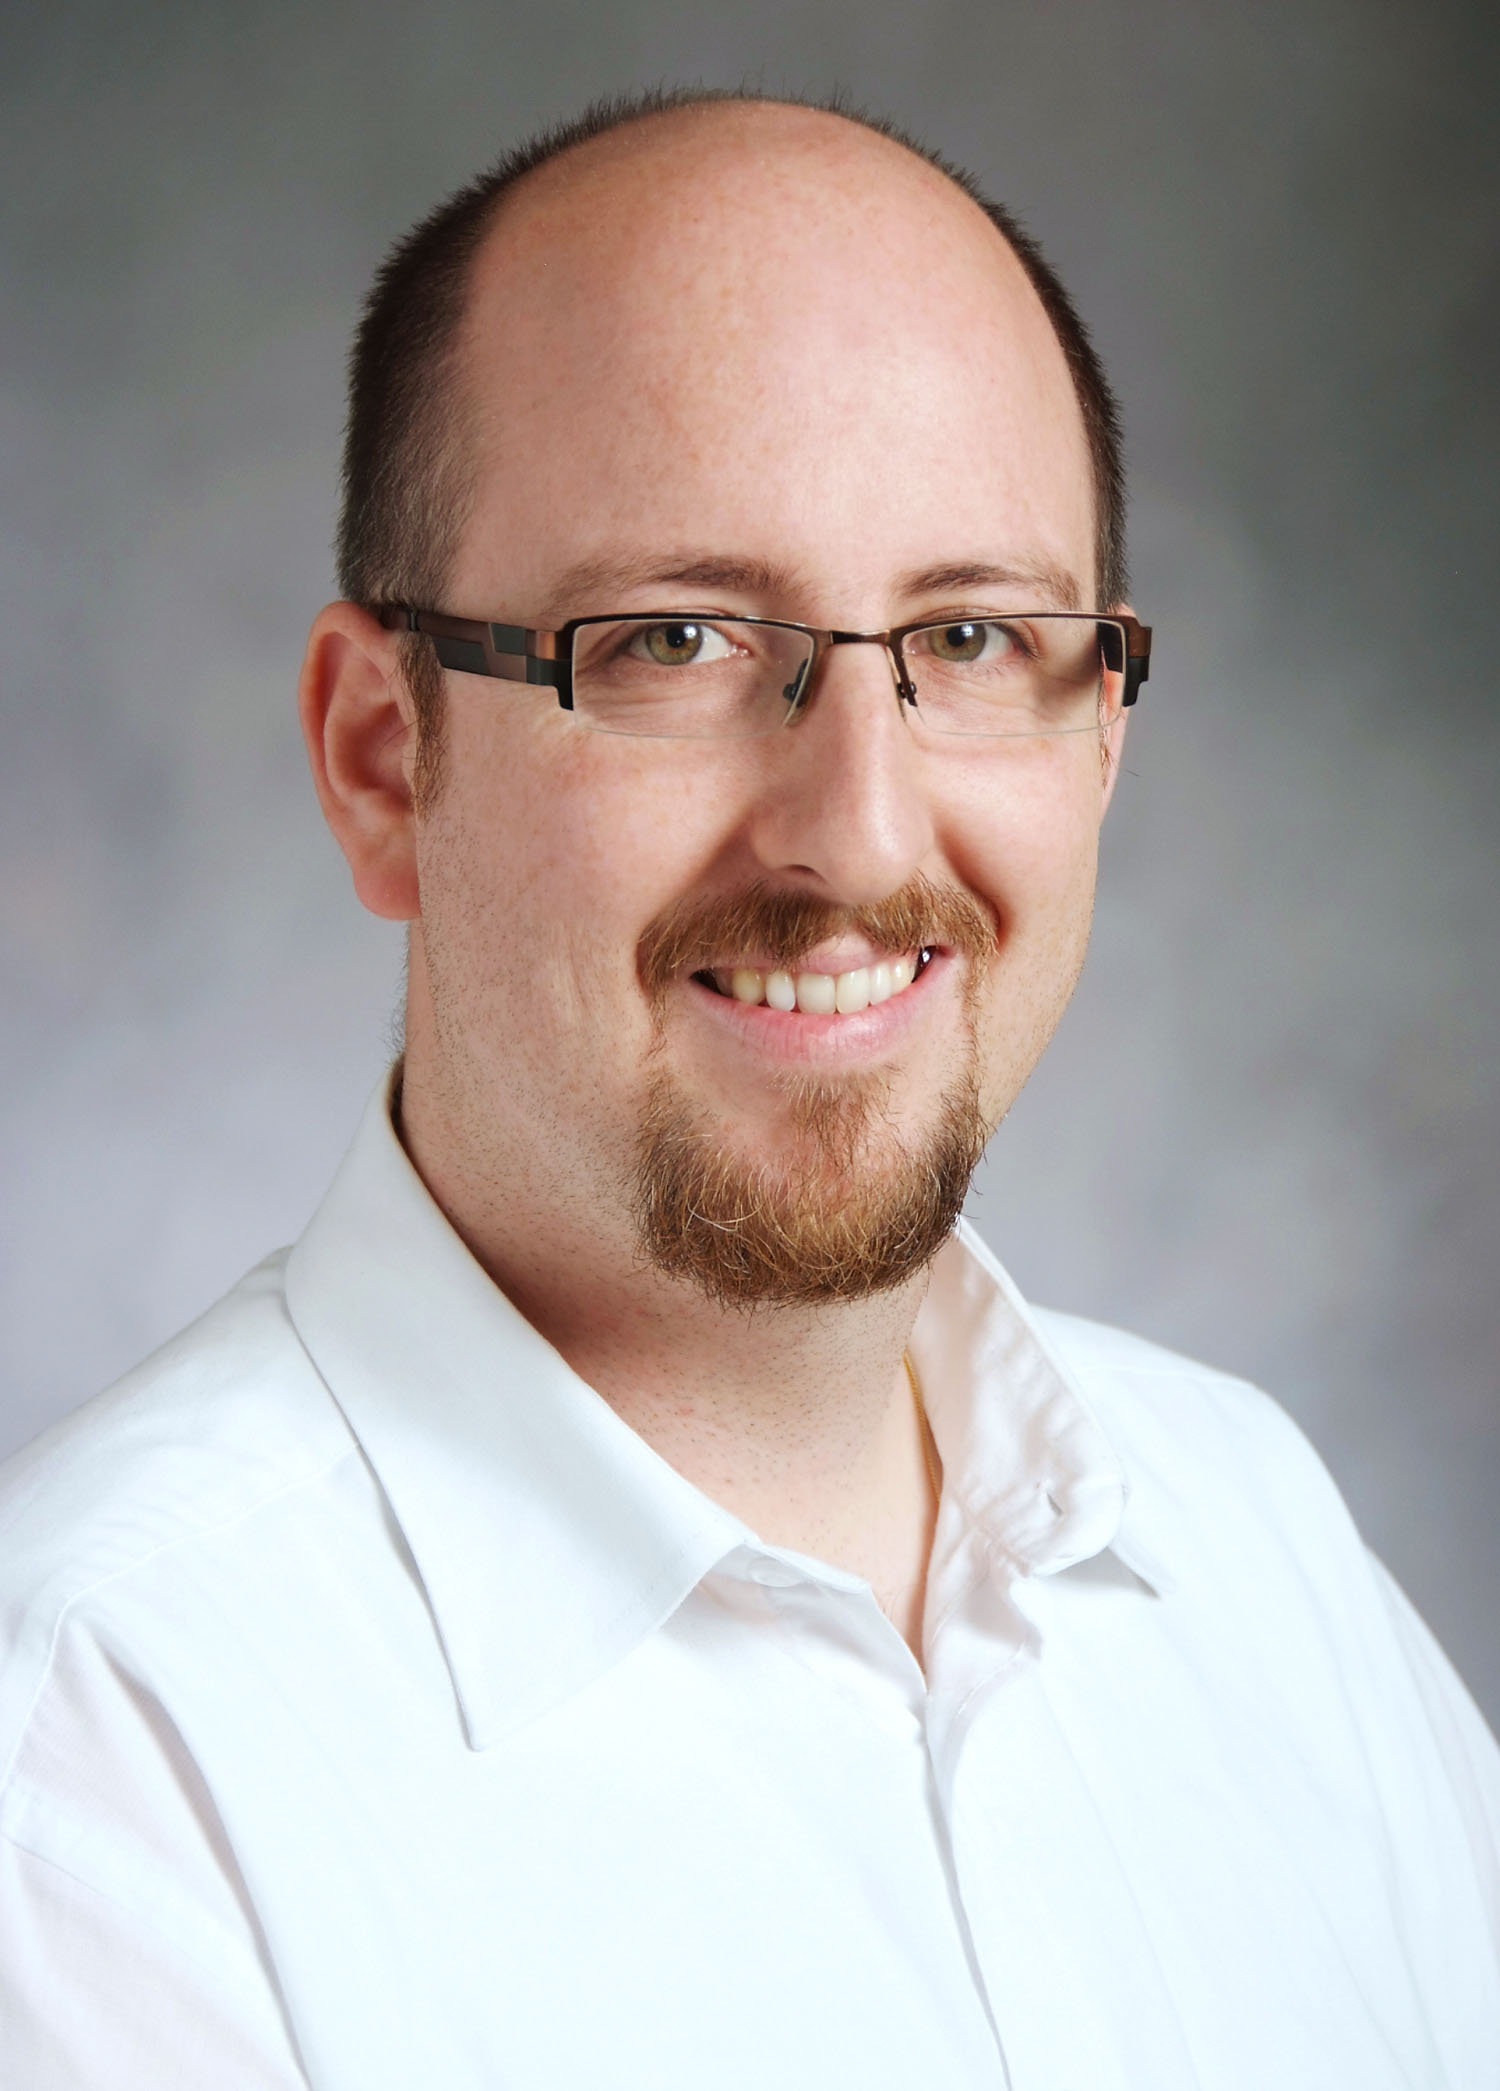
\includegraphics[width=6cm]{images/Landerer_Claudio.jpg}
		\caption{Mag. Claudio Landerer}
	\end{figure}
		
\newpage
\subsection{Partner}
\begin{figure}[H]
	\centering
	
\includegraphics[]{images/ClockstoneLogo.png}
	\caption{ClockStone Softwareentwicklung GmbH}
\end{figure}
Unser Partner während der Diplomarbeit war die Firma ClockStone Softwareentwicklung GmbH. Unser Ansprechpartner war [NAME].
\begin{figure}[H]
	\centering
	\includegraphics[]{images/betreuer.jpg}
	\caption{Mag. Claudio Landerer}
\end{figure}
\subsection{Ansprechpartner}
\section{Vorerhebungen}
\subsection{Projektzieleplan}
Projektziele-Hierarchie - SMART
\subsection{Projektumfeld}
\begin{itemize}
	\item Identifikation der Stakeholder
	\item Charakterisierung der Stakeholder
	\item Maßnahmen
	\item Grafische Darstellung des Umfeldes
\end{itemize}
\subsection{Risikoanalyse}
\begin{itemize}
	\item Risikomatrix
\end{itemize}
\section{Pflichtenheft}
\subsection{Zielbestimmung}
\begin{itemize}
	\item Projektbeschreibung
	\item IST-Zustand
	\item SOLL-Zustand
	\item NICHT-Ziele (Abgrenzungskriterien)
\end{itemize}
\subsection{Produkteinsatz und Umgebung}
\begin{itemize}
	\item Anwendungsgebiet
	\item Zielgruppen
	\item Betriebsbedingungen
	\item Hard-/Softwareumgebung
\end{itemize}
\subsection{Funktionalitäten}
\begin{itemize}
	\item MUSS-Anforderungen
	\begin{itemize}
		\item Funktional
		\item Nicht-funktional
	\end{itemize}
	\item KANN-Anforderungen
	\begin{itemize}
		\item Funktional
		\item Nicht-funktional
	\end{itemize}
\end{itemize}
\subsection{Testszenarien und Testfälle}
\begin{itemize}
	\item Beschreibung der Testmethodik
	\item Testfall 1
	\item Testfall 2
	\item \ldots
\end{itemize}
\subsection{Liefervereinbarung}
\begin{itemize}
	\item Lieferumfang
	\item Modus
	\item Verteilung(Deployment)
\end{itemize}
\section{Planung}
\subsection{Projektstrukturplan}
\subsection{Meilensteine}
\subsection{Gant-Chart}
\subsection{Abnahmekriterien}
\subsection{Pläne zur Evaluierung}
\subsection{Ergänzungen und zu klärende Punkte}

\chapter{Vorstellung des Produktes}


\section{Produktbeschreibung}
Das Computerspiel NeXt ist in den Genres Jump and Run und Puzzle angesiedelt. Hauptaugenmerk dieses Spiels ist das sogenannte „Time-Rift“ Prinzip. Bei diesem Prinzip geht es darum, dass der Spieler jedes Level mehrmals in einzelnen Durchläufen spielen wird. Der Clue an der Sache ist jedoch, dass die zuvor gespielten Charaktere sich genauso bewegen wie sie in den vorigen Durchläufen gesteuert wurden. Das heißt: Hat der Spieler mit dem ersten Charakter einen Schalter betätigt, der eine Tür öffnet, dann wiederholt der Charakter diesen Vorgang, nur diesmal von selbst. Währenddessen kann der Spieler mit dem zweiten Charakter zu der zuvor genannten Tür gehen, welche sich öffnet, da der erste Charakter wieder den Schalter betätigt und somit wird das Level beendet. Durch dieses besondere Spielprinzip können vollkommen neue Puzzele-Elemente in das Produkt eingebaut werden, dies soll den Reiz des Spiels ausmachen.  Damit das Spiel aber nicht zu leicht wird, wird noch ein Zeitfaktor eingebaut, welcher den Spieler unter Druck setzten soll. Schafft der Spieler nicht den Schalter in der geforderten Zeit zu betätigen, so wird er mit dem zweiten Charakter nicht durch die Tür kommen und kann deshalb nicht das Level beenden. Durch ein abwechslungsreiches Level Design und das oben beschriebene Spielprinzip soll ein interessantes Spiel entwickelt werden das auch einen großen Wiederspielfaktor als Ziel hat. Die Benutzeroberfläche so wie das Spielgefühl sollen intuitiv sein und für alle User keine große Umstellung zu anderen Spielen sein. Die genauen Mechaniken sowie die Funktionsweise des Spiels wurden in der Dokumentation erläutert.  



\chapter{Eingesetzte Technologien}
\begin{itemize}
	\item Kurzbeschreibung aller Technologien, die verwendet wurden.
	\item Technologien die aus dem Unterricht bekannt sind, nur nennen und deren  Einsatzzweck im Projekt beschreiben, nicht die Technologien selbst.
	\item Technologien die aus dem Unterricht nicht bekannt sind, im Detail beschreiben incl. deren Einsatz im Projekt
	\item Fokus aus eingesetzten Frameworks
\end{itemize}

\section{Unity-Engine}
\subsection{Spiele-Engine-Erklärung}
Eine Engine ist eine Art Framework 

\chapter{Problemanalyse}
\section{USE-Case-Analyse}
\begin{itemize}
	\item UseCases auf Basis von Benutzerzielen identifizieren: 
	\begin{itemize}
		\item Benutzer eines Systems identifizieren
		\item Benutzerziele identifizieren (Interviews)
		\item Use-Case-Liste pro Benutzer definieren
	\end{itemize}
	\item UseCases auf Basis von Ereignissen identifizieren: 
	\begin{itemize}
		\item Externes Event triggert einen Prozess
		\item zeitliches Event triggert einen Prozess (Zeitpunkt wird erreicht) 
		\item State-Event (Zustandsänderung im System triggert einen Prozess)
	\end{itemize}
	\item Werkzeuge:
	\begin{itemize}
		\item USE-Case-Beschreibungen (textuell, tabellarisch)
		\item USE-Case-Diagramm
		\item Aktivitätsdiagramm für den Use-Case (Interaktion zwischen Akteur und System abbilden)
		\item System-Sequenzdiagramm (Spezialfall eines Sequenzdiagramms: Nur 1 Akteur und 1 Objekt, das Objekt ist das komplette System, es geht um die Input/Output Requirements, die abzubilden sind)
	\end{itemize}
\end{itemize}

\section{Domain-Class-Modelling}
\begin{itemize}
	\item "Dinge" (Rollen, Einheiten, Geräte, Events etc.) identifizieren, um die es im Projekt geht
	\item ER-Modellierung oder Klassendiagramme
	\item Zustandsdiagramme (zur Darstellung des Lebenszyklus von Domain-Klassen darstellen)
\end{itemize}

\section{User-Interface-Design}
\begin{itemize}
	\item Mockups
	\item Wireframes
\end{itemize}


\chapter{Systementwurf}

\section{Architektur}

\subsection{Design der Komponenten}

Darstellung und Beschreibung der Systemarchitektur;

\begin{itemize}
	\item  statische Zerlegung des Systems in seine physischen Bestandteile (Komponenten, Komponentendiagramm)
	\item (textuelle) Beschreibung des dynamischen Zusammenwirkens aller Komponenten 
	\item (textuelle) Beschreibung der Strategie für die Architektur, d. h. wie die Architektur in Statik und Dynamik funktionieren soll.
	\item Verwendung von Referenzarchitekturen bzw. Architekturmustern (als Schablonen, z.B. MVC. Plugin, Pipes and Filters)
	\begin{itemize}
		\item MVC
		\item Schichten
		\item Pipes
		\item Request Broker
		\item Service-Oriented
	\end{itemize}
\end{itemize}

\subsection{Benutzerschnittstellen} 
\begin{itemize}
	\item Design des UIs
	\item Dialoge, Dialogsteuerung, Ergonomie, Gestaltung, Eingabeüberprüfungen
\end{itemize}

\subsection{Datenhaltunskonzept}
\begin{itemize}
	\item Design der Datenbank (ER-Modell)
	\item Design des Zugriffs auf diese Daten (Datenhaltungskonzept)
	\item Caching, Transaktionen
\end{itemize}

\subsection{Konzept für Ausnahmebehandlung}
\begin{itemize}
	\item Systemweite Festlegung, wie mit Exceptions umgegangen wird
	\item Exceptions sind primär aus den Bereichen UI, Persistenz, Workflow-Management
\end{itemize}

\subsection{Sicherheitskonzept}
Beschreibung aller sicherheitsrelevanten Designentscheidungen

\begin{itemize}
	\item Design der Security-Elemente
	\item Design von Safety-Elementen (Fehlertoleranz, Verfügbarkeit etc.)
\end{itemize}

\subsection{Design der Testumgebung}
\begin{itemize}
	\item wie wird getestet (Unit-Testing, Integrationstesting, Systemtests, Akzeptanztests)
	\item Testumgebung, Testprozess, Teststrategie, Testmethoden, Testfälle
\end{itemize}


\subsection{Desing der Ausführungsumgebung}
\begin{itemize}
	\item Deployment (DevOps)
	\item Betrieb (besonders Hoch- und Hertunerfahren der Anwendung)
\end{itemize}

\section{Detailentwurf}

Design jedes einzelnen USE-Cases

\begin{itemize}
	\item Design-Klassendiagramme vom Domain-Klassendiagramm ableiten (incl. detaillierter Darstellung und Verwendung von Vererbungshierarchichen, abstrakten Klassen, Interfaces)
	\item Sequenzdiagramme vom System-Sequenz-Diagramm ableiten
	\item Aktivitätsdiagramme
	\item Detaillierte Zustandsdiagramme für wichtige Klassen
\end{itemize}

Verwendung von CRC-Cards (Class, Responsibilities, Collaboration) für die Klassen
\begin{itemize}
	\item um Verantwortlichkeiten und Zusammenarbeit zwischen Klassen zu definieren und
	\item um auf den Entwurf der Geschäftslogik zu fokussieren
\end{itemize}

Design-Klassen für jeden einzelnen USE-Case können z.B. sein:

\begin{itemize}
	\item UI-Klassen
	\item Data-Access-Klassen
	\item Entity-Klassen (Domain-Klassen)
	\item Controller-Klassen
	\item Business-Logik-Klassen
	\item View-Klassen
\end{itemize}

Optimierung des Entwurfs (Modularisierung, Erweiterbarkeit, Lesbarkeit):

\begin{itemize}
	\item Kopplung optimieren
	\item Kohäsion optimieren
	\item SOLID
	\item Entwurfsmuster einsetzen
\end{itemize}

\chapter{Implementierung}
Detaillierte Beschreibung der Implementierung aller Teilkomponenten der Software entlang der zentralsten Use-Cases:

\begin{itemize}
	\item GUI-Implementierung
	\item Controllerlogik
	\item Geschäftslogik
	\item Datenbankzugriffe
\end{itemize}

Detaillierte Beschreibung der Teststrategie (Testdriven Development):

\begin{itemize}
	\item UNIT-Tests (Funktional)
	\item Integrationstests
\end{itemize}

Zu Codesequenzen:
\begin{itemize}
	\item kurze Codesequenzen direkt im Text (mit Zeilnnummern auf die man in der Beschreibung verweisen kann)
	\item lange Codesequenzen in den Anhang (mit Zeilennummer) und darauf verweisen (wie z.B. hier \cref{qj})
\end{itemize}

\chapter{Deployment}
\begin{itemize}
	\item Umsetzung der Ausführungsumgebung
	\item Deployment
	\item DevOps-Thema
\end{itemize}

\chapter{Tests}

\section{Systemtests} 
\subsection{Einführung}
Nachfolgend sind 4 tabellarisch dargestellte Testfälle beschrieben, welche grundlegende Funktionen des Projekts Darstellen und deren Funktionalität gewährleisten sollen.

\subsection{Testfälle}
\begin{table}
	\caption{Testfall 1: Bewegungssteuerung}
\renewcommand{\arraystretch}{1.5}
\begin{tabular}{|p{3.5cm}|p{11cm}|}
	
	\hline 
	\textbf{Nummer} & 1 \\ 
	\hline 
	\textbf{Name} & {\large Bewegungssteuerung} \\ 
	\hline 
	\textbf{Beschreibung} & 
	Es soll gewährleistet werden, dass die Steuerung der Spielfigur mittels der unten angegebenen Tasten sowie deren Kombination miteinander wie gewünscht funktioniert.  \\ 
	\hline 
	\textbf{Vorbedingung} & 
	\begin{itemize}
		\setlength{\itemsep}{1pt}
		\setlength{\parskip}{0.5pt}
		\item Spiel muss gestartet sein
		\item Level muss gewählt sein
	\end{itemize} \\ 
	\hline 
	\textbf{Tester} & Lukas Vogel \\ 
	\hline 
	\textbf{Datum} & 8.5.2018 \\ 
	\hline 
	\textbf{Vorgehen} & 
	\textit{Soll-Verhalten:}
	\begin{itemize}
		\setlength{\itemsep}{1pt}
		\setlength{\parskip}{0.5pt}
		\item A --> Bewegung der Spielfigur nach links.
		\item D --> Bewegung der Spielfigur nach rechts.
		\item Leertaste --> Vertikale Bewegung der Spielfigur nach oben.
		\item A + Leertaste --> Eine gemischte Bewegung die Horizontal nach links und Vertikal nach oben geht (Sprung nach links).
		\item D + Leertaste --> Eine gemischte Bewegung die Horizontal nach rechts und vertikal nach oben geht (Sprung nach rechts) \newline
	\end{itemize}  
	
	
	\textit{Ist Verhalten:}
	\begin{itemize}
		\setlength{\itemsep}{1pt}
		\setlength{\parskip}{0.5pt}
		\item A --> Spielfigur bewegt sich nach links.
		\item D --> Spielfigur bewegt sich nach rechts.
		\item Leertaste --> Spielfigru bewegt sich vertikal nach oben.
		\item 	A + Leertaste --> Sprung nach links.
		\item D + Leertaste --> Sprung nach rechts.
	\end{itemize}\\ 
	\hline 
	\textbf{Erfolgskriterien} & 
	\textit{Gewünschtes Verhalten:}
	\begin{itemize}
		\setlength{\itemsep}{1pt}
		\setlength{\parskip}{0.5pt}
		\item Flüssige Bewegung ohne Stopps
		\item Bedingte Beeinflussung des Verhaltens durch die Physik-Engine
		\item Tatsächliche Bewegung durch Tastendruck
	\end{itemize} \\ 
	\hline 
\end{tabular} 
\end{table}

\begin{table}
	\caption{Testfall 2: Levelabschluss}
	\renewcommand{\arraystretch}{1.5}
	\begin{tabular}{|p{3.5cm}|p{11cm}|}
		
		\hline 
		\textbf{Nummer} & 2 \\ 
		\hline 
		\textbf{Name} & {\large Levelabschluss} \\ 
		\hline 
		\textbf{Beschreibung} & 
		Es soll gewährleistet werden, dass der Spieler beim Abschließen des Levels in eine Übersicht (Level-Übersicht) gebracht wird. Durch das öffnen der Level-Übersicht kann der User entscheiden ob er ein anders Level öffnen will oder mittels Button ins Hauptmenü der Anwendung. \\ 
		\hline 
		\textbf{Vorbedingung} & 
		\begin{itemize}
			\setlength{\itemsep}{1pt}
			\setlength{\parskip}{0.5pt}
			\item Spiel muss gestartet sein
			\item Level muss gewählt sein
			\item Spieler muss Ende des Levels erreichen
		\end{itemize} \\ 
		\hline 
		\textbf{Tester} & Lukas Vogel \\ 
		\hline 
		\textbf{Datum} & 8.5.2018 \\ 
		\hline 
		\textbf{Vorgehen} & 
		\textit{Soll-Verhalten:}
		\begin{itemize}
			\setlength{\itemsep}{1pt}
			\setlength{\parskip}{0.5pt}
			\item Beim Levelabschluss kommt ein Overlay, das 2 Möglichkeiten bieten (Nächstes Level, Hauptmenü)
			\item Wird einer der Levelbuttons (nummerierte Quadrate) betätigt, startet das gewünschte Level. 
			\item Der Button „Back“ bringt den Spieler in das Hauptmenü des Spieles. \newline
		\end{itemize}  
		
		
		\textit{Ist Verhalten:}
		\begin{itemize}
			\setlength{\itemsep}{1pt}
			\setlength{\parskip}{0.5pt}
			\item Wechsel in die Levelübersicht nach Abschluss des Levels
			\item Wird Levelbutton gedrückt startet richtiges Level
			\item Back-Button öffnet Hauptmenü 
		\end{itemize}\\ 
		\hline 
		\textbf{Erfolgskriterien} & 
		\textit{Gewünschtes Verhalten:}
		\begin{itemize}
			\setlength{\itemsep}{1pt}
			\setlength{\parskip}{0.5pt}
			\item 	Der Spieler soll durch das Overlay die Auswahlmöglichkeit haben, weiter zu spielen oder zurück ins Hauptmenü zu navigieren.
		\end{itemize} \\ 
		\hline 
	\end{tabular} 
\end{table}

\begin{table}
	\caption{Testfall 3: Tod der Spielfigur durch Fall}
	\renewcommand{\arraystretch}{1.5}
	\begin{tabular}{|p{3.5cm}|p{11cm}|}
		
		\hline 
		\textbf{Nummer} & 3 \\ 
		\hline 
		\textbf{Name} & {\large Tod der Spielfigur durch Fall} \\ 
		\hline 
		\textbf{Beschreibung} & 
		Bei einem Fehler des Spielers, indem er durch falsches Steuern des Charakters aus der Spielwelt fällt, wird der Charakter wieder zur Startposition zurückgesetzt. \\ 
		\hline 
		\textbf{Vorbedingung} & 
		\begin{itemize}
			\setlength{\itemsep}{1pt}
			\setlength{\parskip}{0.5pt}
			\item Spiel muss gestartet sein
			\item Level muss gewählt sein
			\item Spieler fällt aus der Spielwelt
		\end{itemize} \\ 
		\hline 
		\textbf{Tester} & Michael Leitner \\ 
		\hline 
		\textbf{Datum} & 8.5.2018 \\ 
		\hline 
		\textbf{Vorgehen} & 
		\textit{Soll-Verhalten:}
		\begin{itemize}
			\setlength{\itemsep}{1pt}
			\setlength{\parskip}{0.5pt}
			\item Charakter wird ab einer bestimmten Grenze („Deathzone“) an den Startpunkt des Levels zurückgesetzt („Respawn“).\newline
		\end{itemize}  
		
		
		\textit{Ist Verhalten:}
		\begin{itemize}
			\setlength{\itemsep}{1pt}
			\setlength{\parskip}{0.5pt}
			\item Respawn der Spielfigur funktioniert. 
		\end{itemize}\\ 
		\hline 
		\textbf{Erfolgskriterien} & 
		\textit{Gewünschtes Verhalten:}
		\begin{itemize}
			\setlength{\itemsep}{1pt}
			\setlength{\parskip}{0.5pt}
			\item Durch das zurücksetzten des Charakters soll ein reibungsloses weiterspielen möglich sein.
		\end{itemize} \\ 
		\hline 
	\end{tabular} 
\end{table}

\begin{table}
	\caption{Testfall 4: Schalter zum Öffnen einer Tür}
	\renewcommand{\arraystretch}{1.5}
	\begin{tabular}{|p{3.5cm}|p{11cm}|}
		
		\hline 
		\textbf{Nummer} & 4 \\ 
		\hline 
		\textbf{Name} & {\large Schalter zum Öffnen einer Tür} \\ 
		\hline 
		\textbf{Beschreibung} & 
		Beim Betätigen des Schalters mittels der Spielfigur, soll eine Tür/Passage geöffnet werden, welche für denn weiteren Spielverlauf wichtig ist. \\ 
		\hline 
		\textbf{Vorbedingung} & 
		\begin{itemize}
			\setlength{\itemsep}{1pt}
			\setlength{\parskip}{0.5pt}
			\item Spiel muss gestartet sein
			\item Level muss gewählt sein
			\item Spieler ist bei einem Schalter
		\end{itemize} \\ 
		\hline 
		\textbf{Tester} & Michael Leitner \\ 
		\hline 
		\textbf{Datum} & 8.5.2018 \\ 
		\hline 
		\textbf{Vorgehen} & 
		\textit{Soll-Verhalten:}
		\begin{itemize}
			\setlength{\itemsep}{1pt}
			\setlength{\parskip}{0.5pt}
			\item Spieler bewegt Spielfigur auf den Schalter
			\item Tür öffnet sich, sobald der Schalter betätigt wurde.\newline
		\end{itemize}  
		
		
		\textit{Ist Verhalten:}
		\begin{itemize}
			\setlength{\itemsep}{1pt}
			\setlength{\parskip}{0.5pt}
			\item Spieler benutzt Schalter und Tür geht auf. 
		\end{itemize}\\ 
		\hline 
		\textbf{Erfolgskriterien} & 
		\textit{Gewünschtes Verhalten:}
		\begin{itemize}
			\setlength{\itemsep}{1pt}
			\setlength{\parskip}{0.5pt}
			\item Durch das öffnen der Tür sollen neue Gebiete des Levels erschlossen werden, um auch letztendlich das Level abzuschließen zu können
		\end{itemize} \\ 
		\hline 
	\end{tabular} 
\end{table}

\section{Akzeptanztests}

\chapter{Projektevaluation}
siehe Projektmanagement-Unterricht

\chapter{Benutzerhandbuch} 
falls im Projekt gefordert

\chapter{Betriebswirtschaftlicher Kontext}
BW-Teil

\chapter{Zusammenfassung}
\section{Projektevaluation}
Während des Projektes lernten wir schnell das wir den Arbeitsaufwand des Projektes überschätzt hatten, am besten wäre es, wenn man sich während den Verschiedenen Ferien mindestens für mehrere Tage getroffen hätte und dann intensiv gearbeitet hätte. Schlussendlich ist das Projekt zwar trotzdem fertiggestellt worden und es erfüllt auch die gewünschten Anforderungen, jedoch war so viel mehr Arbeit zusätzlich zu dem normalen Schultag nötig. 

Die Zusammenarbeit des Teams war nie ein Problem, dass einzige was hierbei ein Rückschlag war, war das ausfallen eines Teammitglieds und die dadurch entstandene zusätzliche Arbeit. Da wir durch diesen Ausfall die Verteilung der Themen sowie die Organisation als Projektteam nochmals neu überdenken mussten. 

Auch bei der Zuordnung der Themen traten keine Probleme auf, da jeder im Team seinen wunschschwerpunkt ohne Diskussion bekam. Dies ist darauf zurück zu führen, dass wir diesbezüglich unterschiedlich sind und es bei diesem Projekt genau passte.
Die größte Schwierigkeit war das Zeitmanagement, da das gesamte Team nicht nur die Diplomarbeit bearbeiten musste, sondern zusätzlich noch die benötigten schulischen Leistungen erbringen musste. Dies führte des Öfteren zu Komplikationen und somit auch zu zeitlichen Verschiebungen von Meilensteinen.

Besonders hervorzuheben ist die Vielfalt an neuen Erfahrungen, die wir während des Projektes sammeln konnten. Wir lernten den gesamten Umfang eines Projekts kennen und welche Arbeitsschritte für ein solches Unterfangen notwendig sind, sei es nur die ständige Kommunikation mit den Teammitgliedern bis zur Fertigung einer umfangreichen Projektdokumentation.

Kosten sind für das Projekt insofern keine entstanden, da wir die benötigte Software komplett ohne Ausgaben bekommen haben. Die einzigen Kosten waren Zeit und Arbeit.

\section{Produktevaluierung}
Sollzustand\newline
Es soll ein Spiele-Prototyp entwickelt, der die vorgegebenen Funktionen realisiert. Das Spiel wird vollständig spielbar sein und einige Levels enthalten, die das Spielprinzip voll zur Geltung bringen. Die Software wird in einer Beta-Phase mit Usern getestet, deren Feedback zur Verbesserung des Spiels verwendet wird. Das Spiel wird als voll funktionsfähiges Spiel an den Auftraggeber übergeben.

Istzustand\newline
Es wurde ein Prototyp entwickelt, der alle vorgegebenen Funktionen realisierte. Das Spiel ist vollständig spielbar und ist mit 4 Level ausgestattet. In diesen Level kommt das grundlegende Spielprinzip zur Geltung. Es wurde auf die Beta-Phase verzichtet, aus dem Grund, dass keine Zeit mehr für einen durchlauf einer Beta-Testphase sowie die Einarbeitung der Ergebnisse des Feedbacks, war. Wegen dem Verlassen eines Projektmitgliedes wurde bei dem Spiel gänzlich auf Soundeffekte und Hintergrundmusik verzichtet. Ebenso wurde die Grafik sehr primitiv gehalten, da das Erstellen von neuen Grafiken sehr aufwendig ist und wir dafür eine zusätzliche Einarbeitungsphase benötigt hätten.

\section{Resümee}
\subsection{Resümee (Leitner Michael)}
Die Entwicklung eines Spieles war ein größerer Aufwand als erwartet.

Gründe dafür sind:
\begin{enumerate}
	\item Für die ausgewählte Engine war eine intensivere Einarbeitung in die Dokumentation notwendig, um auch die Engine ohne Probleme verwenden zu können.
	\item Der Absprung eines Projektmitgliedes hatte uns mehr Arbeit beschert, aber durch Absprache mit dem Projektpartner und Projektbetreuer, wurde der Projektumfang angepasst.
	\item Das komplette Diplomprojekt neben dem normalen Schultag durchzuführen und erarbeiten, war ebenso ein Faktor, der sich schwer auf das Zeitmanagement gelegt hat.
\end{enumerate}
	
Letztendlich ist aber alles im Projekt, mehr oder weniger, gut verlaufen. Des Weiteren habe ich viel für die Spiele Entwicklung gelernt, dass ich für zukünftige Projekte (ob privat oder beruflich) anwenden kann. Die Arbeitsaufteilung war zwischen Lukas Vogel und mir sehr gerecht und beide hatten ungefähr den gleichen Aufwand. Für alle die ein Spiel entwickeln möchten gebe ich nur einen Tipp auf dem Weg: „Plant euch genug Zeit ein. Es hat einen Grund, warum so viele Veröffentlichungen von Spiele verschoben werden.“.

\subsection{Resümee (Vogel Lukas)}
Während der Diplomarbeit lernte ich den Ablauf eines Projekts haut nah kennen und konnte somit viele wertvolle Erfahrungen sammeln, welche mir sicherlich auch in Zukunft helfen werden.

Die ersten Neuerungen für mich waren die vielen verschieden Programme, die wir im Laufe unsers Projekts verwendeten. Eine Software, die für mich komplett neu war, war Latex mit der wir die Diplomarbeit dann geschrieben haben. Ein Textverarbeitungsprogramm in der man die Formatierung „programmiert“ war etwas Ungewohntes, jedoch ist das Programm perfekt auf wissenschaftliche Arbeiten wie Diplomarbeiten zugeschnitten und zeigte uns einige Vorteile gegenüber anderer Applikationen.  

Mitten während des Projekts lernten wir wie wichtig es ist immer einen Plan-B zu haben, da eine Teammitglied die das IT-Kolleg frühzeitig beendete und wir somit ein Teammitglied weniger waren. Dies hat die Folge mit sich das wir die Aufteilung sowie den Umfang des Projekts noch einmal komplett überdenken mussten. 

Besonders interessant war das Kennenlernen der Spieleentwicklung und dadurch einen Überblick zu bekommen wieviel Arbeit hinter so einer Software steht. Das erste große Thema war die Einarbeitung in eine komplett fremde Programmierumgebung. Natürlich hatten wir mit der Programmiersprache C\# schon während unser Unterrichts zu tun, jedoch ist das Programmieren mit C\# in Kombination mit der Spiele-Engine Unity nochmal etwas ganz anderes. Was mir dabei aber auffiel war, dass nach der Lernphase und der Eingewöhnungszeit in die neue Entwicklungsumgebung von Unity, auch hier wieder einige Parallelen mit den im Unterricht besprochen Themen zu ziehen waren. Man darf aber an dieser Stelle nicht glauben, dass das entwickeln mit Unity dem normalen Programmieren von Anwendungen stark ähnelt, da Unity auf eine ganz eigene Art funktioniert.

Die größte Aufgabe war eindeutig das Zeitmanagement. Das Problem war, zusätzlich zu den vielen Unterrichtseinheiten und die Zeit, die für das Lernen oder das erledigen anderer wichtiger schulischer Tätigkeiten war, noch Zeit für das Projekt zu finden. Diese Schule fordert einen mehr als wie alle anderen die ich davor besucht habe und zusätzlich kommt dann noch die Diplomarbeit hinzu. Es gab nicht nur einmal den Punkt, an dem ich nicht mehr wusste wie ich alles erledigen sollte. 
Abschließend ist nur zu sagen das es eine besondere Herausforderung war diese Diplomarbeit zu erstellen und ich sehr viel fürs Leben dazugelernt habe.
